\section{Hardware}
%The quadcopter has been provided by Aalborg university and professor Henrik Shjøiler\fixme{add danish letters}. This chapter has the purpose of describing the hardware. 
%The hardware is tested and the results of these test will be presented. 
The hardware used to develop this project consists of the quadcopter and the Vicon system that is used as a sensor. In this section, the most relevant hardware is explained in more detail.

\subsection{Motor and Propeller}
The quadcopter is equipped with four brushless outrunner motors named Turnigy Multistar. 

Brushless motors are electric powered with a DC power that require a electronic commutator, which generates a sinusoidal or trapezoidal waveform, to run the motor. They have a higher power density and higher reliability than conventional DC motors.

Within this kind, outrunner motors have their magnets in the outer shell, the rotor. The rotor spins around the fixed coils that form the stator. Due to the more space in the rotor for magnets, they normally have more poles that inrunner motors, and thus, are able to produce more torque for the same size.  

The motor used has a $k_v$ of 935 $rpm/V$, 14 poles and maximum current of 15 $A$. \fxnote{Source: \url{https://www.hobbyking.com/en_us/mt2213-935kv-multistar-motor-and-propeller-combo-10x4-5-cw-ccw.html}}

The motor used is shown in \autoref{fig:Motor}.
\begin{figure}[H]
	\centering
	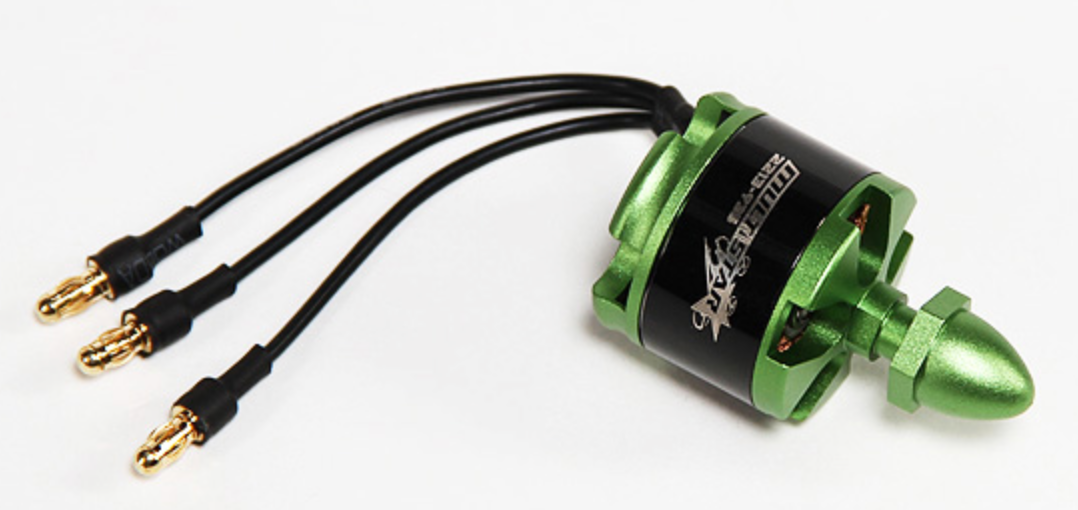
\includegraphics[scale=0.5]{figures/motor.png}
	\caption{One of the four motors mounted on the quadcopter.}
	\label{fig:Motor}
\end{figure} 

The propellers are sold with the motors and are 10 inches long (25.4 cm) and has a pitch of 4.5 (11,43 cm) inches. The pitch is the distance traveled by a propeller after one complete rotation. For this to be true the propeller must turn inside a solid surface, the traveled distance is less if it rotates inside a liquid or gas. \fxnote{Source: \url{ http://www.propellerpages.com/?c=articles&f=2006-03-08_what_is_propeller_pitch}} A higher pitch creates more turbulence and make the quadcopter less steady when flying.\fxnote{Source: \url{https://oscarliang.com/quadcopter-motor-propeller/}} 

The length of the propeller is proportional to the efficiency of the quadcopter. Hence, a longer propeller has an increase in maximum speed. The acceleration of a small propeller is greater than that of a larger propeller. Thus it is easier to change the inertia of moment if utilizing a small propeller compared to a larger one. \fxnote{source: \url{https://oscarliang.com/quadcopter-motor-propeller/}} 

In this case a propeller which is 10 inches long and has a pitch of 4.5 is suitable for the utilized quadcopter, as it has been utilized in multiple cases before. 

A picture of the utilized propellers can be seen in \autoref{fig:Propeller}.

\begin{figure}[H]
	\centering
	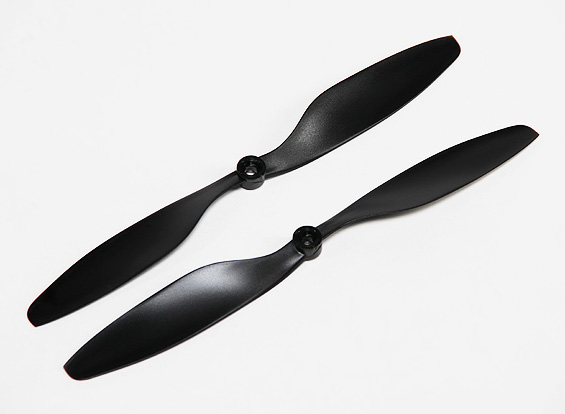
\includegraphics[scale=0.4]{figures/propeller.png}
	\caption{Two of the four propellers mounted on the quadcopter's motors.}
	\label{fig:Propeller}
\end{figure}

%The relationship between PWM signal to the motor controllers and the velocity of the propeller can be seen in Figure ZZ. \fxnote{pull diagram from measurement report}

%It has been observed during tests, that the motor runs faster as it's temperature increases. This is not expected due to the increased resistance, that occurs when the coils within the motor are heated. Therefore the relationship between PWM signal and velocity is not representative for all cases. It is however deemed reasonable to neglect this variance and presume a relationship as it is derived in the measurement report, see Appendix YY.
 
\subsection{Motor Controller}
The quadcopter comes with four electronic speed controllers, ESCs, one for each motor. The ESCs produce an 8 kHz PWM, are rated for a 2-4 cell Li-Po battery and can handle a constant current of up to 30 A. The ESCs also has a 5.5 V, 4 A output for powering e.g. a controller board.\cite{HKing}

\begin{figure}[H]
	\centering
	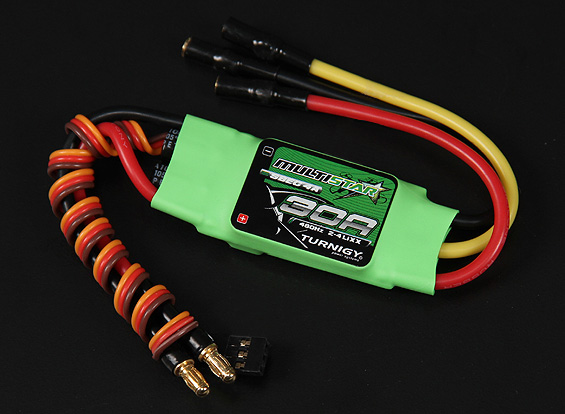
\includegraphics[scale=0.4]{figures/ESC}
	\caption{One of the four Electronic Speed Controllers mounted on the quadcopter.\cite{HKing}}
	\label{fig:esc}
\end{figure}
\subsection{Processor}
The implementation of the controllers is done in a microprocessor from Atmel, the ATmega2560, mounted in the ArduinoMEGA development board, as seen in figure \autoref{fig:ATmega}.

This processor has up to 16 PWM output channels, two 8-bit timers and four 16-bit timers, four USART modules, 8 kilobytes of internal memory and a processing speed of 16 MIPS. With this capabilities, a quadcopter control could be implemented.

The use of the development board makes the use of the wireless modules easier as an arduino shield can be directly plugged in. Furthermore, it allows a faster set up of the microcontroller as all required hardware (oscillatior, power supply, etc.) is already present in the board. 
\begin{figure}[H]
	\centering
	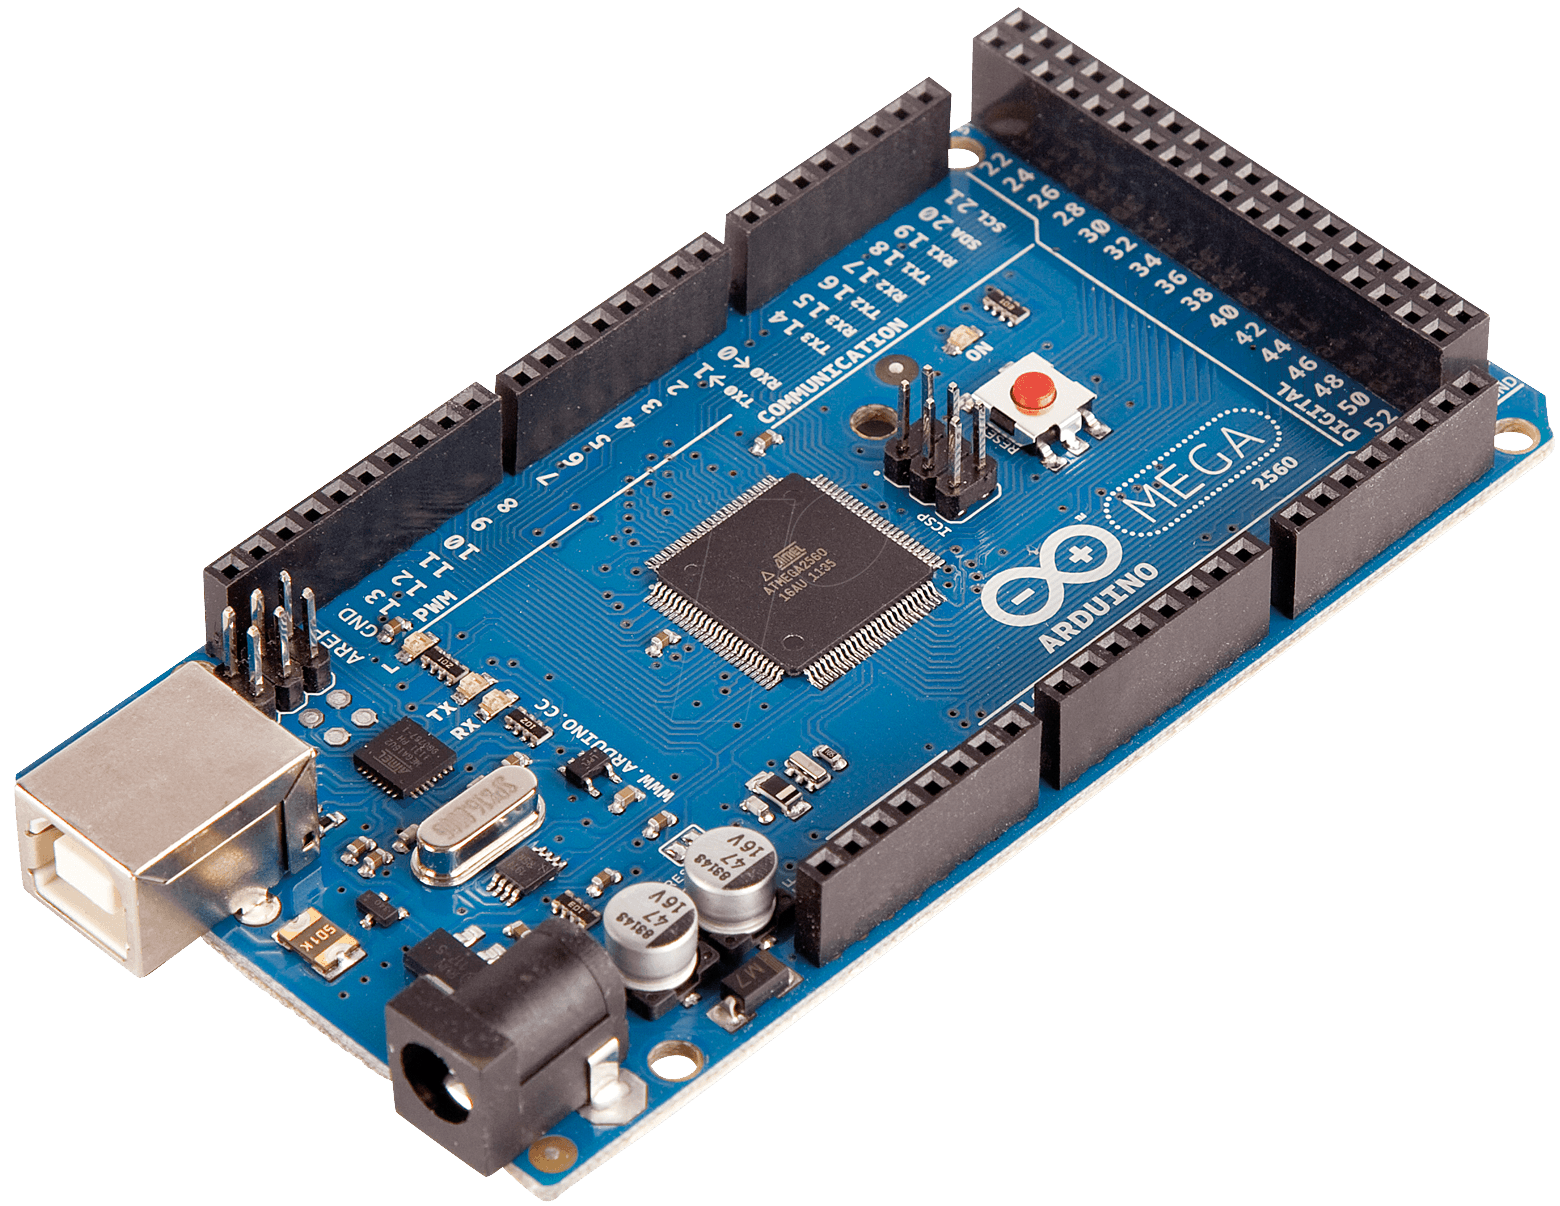
\includegraphics[scale=0.17]{figures/ARDUINO_MEGA}
	\caption{AtMega2560 mounted in the ArduinoMEGA development board.}
	\label{fig:ATmega}
\end{figure}
\subsection{Wireless Modules}
The wireless modules used to communicate with the quadcopter are called XBEE, see \autoref{fig:XBEE}. They communicate at a 2.4 GHz frequency and they take care of all communication layers but the transport layer protocol. In order to use this modules, the packet has to be sent through the serial port when using the computer or through the USART module when using the microcontroller. 
\begin{figure}[H]
	\centering
	\includegraphics[scale=0.4]{figures/XBEE}
	\caption{XBEE wireless modules.}
	\label{fig:XBEE}
\end{figure}

\subsection{Battery}
The battery available for the prototype, is a Zippy Flightmax battery. It weighs 141 gram, has a capacity of 1500 mAh, a voltage of 11.1 volts and a discharge current of 20 amperes.

%removed by Niels: It shall be noted, that the battery level...
The battery level drops over time, with a significance that can not be neglected as it may have great impact on the output of the motor and therefore on the lift of the propeller. It is possible to measure the battery level while operating the quadrotor. By taking into account the battery level in the test of the PWM signal to velocity, it is possible to obtain a quadcopter having constant lift force, if this is requested\fxnote{Niels and Alejandro suggest: With this information and knowledge of the relationship between voltage and RPM it is possible to account for the battery level, and thereby rectify the problem. [ref to test - maybe - should the test be discussed this early?]}.

\subsection{Vicon System}
The Vicon system is a powerful tool that provides real-time position and orientation data captured with 9 infrared cameras.This information can be used to track objects inside the room the system is built in.
%An example is found in Aalborg University as seen in \figref{ViconRoom}. 

%\begin{figure}[H]
%	\centering
%	\includegraphics[scale=0.5]{figures/ViconRoom}
%	\caption{Aalborg University's Vicon room.}
%	\label{ViconRoom}
%\end{figure}

To use this system, markers are attached to the object that is to be tracked. The Vicon system streams the position of the markers and the position and orientation of the object at 100 Hz for a computer to read them. The data can be received by using an SDK plugin for MATLAB. In this way, data can be operated in the MATLAB environment, making it easier to obtain variable derivatives like velocities or accelerations.

The user interface of the Vicon system is shown in \autoref{fig:ViconTracker}. 
\begin{figure}[H]
	\centering
	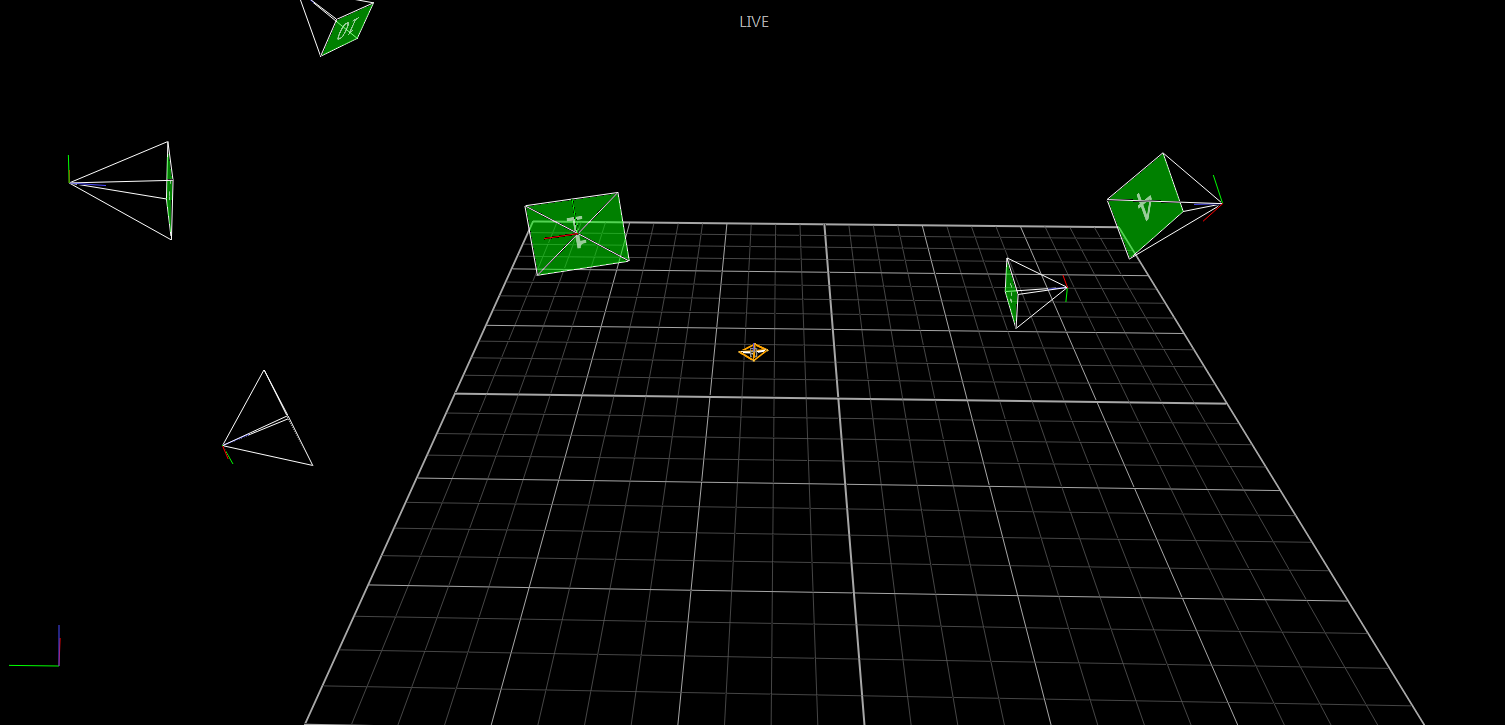
\includegraphics[scale=0.27]{figures/ViconTracker}
	\caption{User interface of the Vicon System, the Vicon Tracker. An object has been created from the markers placed on the drone.}
	\label{fig:ViconTracker}
\end{figure}
It is called Vicon Tracker and it allows the creation of objects by grouping markers present in the room. It also allows to change the center of gravity of the created objects and rotate the inertial and body reference frames to any desired orientation.